\documentclass{article}

% content/resources/templates/preamble.tex
\usepackage[margin=0.6in]{geometry}
\author{Milav Dabgar}
\usepackage{amsmath,amssymb,amsthm}
\usepackage{booktabs}
\usepackage{multirow}
\usepackage{xcolor}
\usepackage{tcolorbox}
\tcbuselibrary{breakable,skins}
\usepackage[colorlinks=true,linkcolor=blue]{hyperref}
\usepackage{titlesec}
\usepackage{enumitem}
\usepackage{tikz}
\usepackage{pgfplots}
\usepackage{circuitikz}
\usepackage[version=4]{mhchem}
\usepackage{longtable}
\usepackage{array}
\usepackage{float}
\usepackage{caption}
\usepackage{listings}

\lstset{
  basicstyle=\small\ttfamily,
  breaklines=true,
  breakatwhitespace=false,
  postbreak=\mbox{\textcolor{red}{$\hookrightarrow$}\space},
  float=false,
  numbers=left,
  numberstyle=\tiny\color{gray},
  numbersep=10pt,
  xleftmargin=2em,
  keywordstyle=\color{blue},
  commentstyle=\color{green!60!black},
  stringstyle=\color{purple},
  backgroundcolor=\color{gray!5},
  showstringspaces=false,
  tabsize=2,
  captionpos=b,
  keepspaces=true,
  columns=flexible
}

\pgfplotsset{compat=1.18}
\usetikzlibrary{shapes,arrows,positioning,calc,patterns,decorations.pathmorphing,decorations.markings,arrows.meta}

% Color scheme
\definecolor{headcolor}{RGB}{0,102,204}
\definecolor{keycolor}{RGB}{220,20,60}
\definecolor{solutioncolor}{RGB}{34,139,34}
\definecolor{mnemoniccolor}{RGB}{148,0,211}
\definecolor{codecolor}{RGB}{0,0,100}

% Spacing
\setlength{\parskip}{3pt}
\setlist[itemize]{nosep}
\setlist[enumerate]{nosep}

% Title formatting
\titleformat{\section}{\Large\bfseries\color{headcolor}}{\thesection}{1em}{}
\titleformat{\subsection}{\large\bfseries\color{headcolor}}{\thesubsection}{1em}{}

% Pandoc tightlist compatibility
\providecommand{\tightlist}{%
  \setlength{\itemsep}{0pt}\setlength{\parskip}{0pt}}

% Pandoc longtable compatibility
\newcounter{none}
\def\thenone{}


% content/resources/templates/english-boxes.tex

% Custom environments
\newtcolorbox{solutionbox}{
 breakable,
 enhanced,
 colback=solutioncolor!5!white,
 colframe=solutioncolor!75!black,
 fonttitle=\bfseries,
 title=Solution
}

\newtcolorbox{solutionboxnobreak}{
 colback=solutioncolor!5!white,
 colframe=solutioncolor!75!black,
 fonttitle=\bfseries,
 title=Solution
}

\newtcolorbox{keyformula}{
 breakable,
 enhanced,
 colback=keycolor!5!white,
 colframe=keycolor!75!black,
 fonttitle=\bfseries,
 title=Key Formula
}

\newtcolorbox{mnemonicboxenv}{
 breakable,
 enhanced,
 colback=mnemoniccolor!5!white,
 colframe=mnemoniccolor!75!black,
 fonttitle=\bfseries,
 title=Mnemonic
}

\newcommand{\mnemonicbox}[1]{%
  \begin{mnemonicboxenv}
    #1
  \end{mnemonicboxenv}
}


% Custom commands for GTU solutions
% This file defines semantic commands for consistent formatting

% Question command with automatic formatting
\newcommand{\question}[2]{%
  \section*{Question #1}%
  \textbf{#2}%
}

% OR question variant
\newcommand{\questionor}[2]{%
  \section*{Question #1 OR}%
  \textbf{#2}%
}

% Proper table environment with caption
\newenvironment{answertable}[1]{%
  \begin{table}[htbp]
  \centering
  \caption{#1}
}{%
  \end{table}
}

% Proper figure environment for diagrams
\newenvironment{answerdiagram}[1]{%
  \begin{figure}[htbp]
  \centering
  \caption{#1}
}{%
  \end{figure}
}

% Semantic markup for key terms
\newcommand{\keyword}[1]{\textbf{#1}}
\newcommand{\code}[1]{\texttt{#1}}
\newcommand{\classname}[1]{\texttt{#1}}
\newcommand{\methodname}[1]{\texttt{#1}}

% Proper quotation marks
\newcommand{\mnemonic}[1]{``#1''}


\usetikzlibrary{shapes.geometric, arrows.meta}

\title{Python Programming (4311601)}
\date{Winter 2023}

\begin{document}
\maketitle

\questionmarks{Question 1(a)}{03}{What is Flow chart? List out symbols used in Flow chart.}

\begin{solutionbox}
A \keyword{flowchart} is a graphical representation of an algorithm that shows the sequence of steps and decision points in a process using standardized symbols.

\begin{answertable}{Flowchart Symbols Table}
\begin{tabulary}{\linewidth}{|l|l|L|}
\hline
\textbf{Symbol} & \textbf{Name} & \textbf{Purpose} \\
\hline
Oval & Terminal & Start/End of program \\
\hline
Rectangle & Process & Processing/Calculation steps \\
\hline
Diamond & Decision & Conditional statements \\
\hline
Parallelogram & Input/Output & Data input or output \\
\hline
Circle & Connector & Connect flowchart parts \\
\hline
Arrow & Flow line & Direction of flow \\
\hline
\end{tabulary}
\end{answertable}

\textbf{Key Points:}
\begin{itemize}
    \item \textbf{Visual representation}: Shows program logic graphically
    \item \textbf{Step-by-step}: Displays sequential flow of operations
    \item \textbf{Decision making}: Diamond symbols show conditional branches
\end{itemize}

\begin{mnemonicbox}\mnemonic{Flow Charts Show Program Steps Visually}\end{mnemonicbox}
\end{solutionbox}

\questionmarks{Question 1(b)}{04}{Write a short note on for loop.}

\begin{solutionbox}
The \keyword{for loop} is used to iterate over a sequence (list, tuple, string, range) in Python.

\begin{answertable}{For Loop Table}
\begin{tabulary}{\linewidth}{|l|l|l|}
\hline
\textbf{Component} & \textbf{Syntax} & \textbf{Example} \\
\hline
Basic & \code{for variable in sequence:} & \code{for i in range(5):} \\
\hline
Range & \code{range(start, stop, step)} & \code{range(1, 10, 2)} \\
\hline
List & \code{for item in list:} & \code{for x in [1,2,3]:} \\
\hline
String & \code{for char in string:} & \code{for c in "hello":} \\
\hline
\end{tabulary}
\end{answertable}

\textbf{Simple Code Example:}
\begin{lstlisting}[language=Python]
for i in range(3):
    print(i)
# Output: 0, 1, 2
\end{lstlisting}

\textbf{Key Features:}
\begin{itemize}
    \item \textbf{Automatic iteration}: No manual counter needed
    \item \textbf{Sequence traversal}: Works with any iterable object
    \item \textbf{Range function}: Creates number sequences easily
\end{itemize}

\begin{mnemonicbox}\mnemonic{For Loops Iterate Through Sequences}\end{mnemonicbox}
\end{solutionbox}

\questionmarks{Question 1(c)}{07}{Write a program to display Fibonacci series up to nth term where n is provided by the user.}

\begin{solutionbox}
\textbf{Fibonacci Series Program:}
\begin{lstlisting}[language=Python]
# Get number of terms from user
n = int(input("Enter number of terms: "))

# Initialize first two terms
a, b = 0, 1

# Display first term
if n >= 1:
    print(a, end=" ")
    
# Display second term
if n >= 2:
    print(b, end=" ")

# Generate remaining terms
for i in range(2, n):
    c = a + b
    print(c, end=" ")
    a, b = b, c
\end{lstlisting}

\textbf{Algorithm Flow:}
\begin{center}
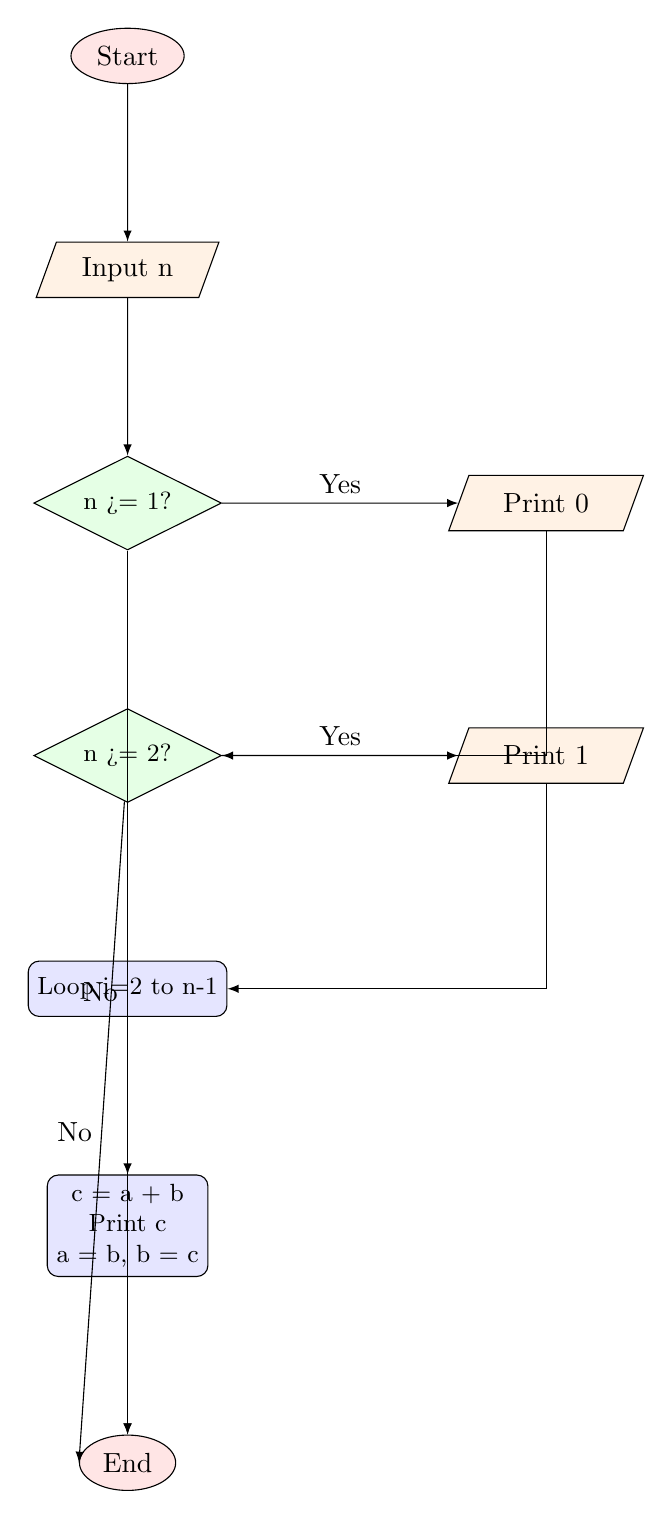
\begin{tikzpicture}[node distance=2cm, auto]
    \node[draw, ellipse, fill=red!10, align=center, minimum height=2em] (start) {Start};
    \node[trapezium, trapezium left angle=70, trapezium right angle=110, draw, fill=orange!10, align=center, minimum height=2em, below=of start] (input) {Input n};
    \node[diamond, draw, fill=green!10, align=center, aspect=2, font=\small, below=of input] (cond1) {n >= 1?};
    \node[trapezium, trapezium left angle=70, trapezium right angle=110, draw, fill=orange!10, align=center, minimum height=2em, right=3cm of cond1] (print0) {Print 0};
    \node[diamond, draw, fill=green!10, align=center, aspect=2, font=\small, below=of cond1] (cond2) {n >= 2?};
    \node[trapezium, trapezium left angle=70, trapezium right angle=110, draw, fill=orange!10, align=center, minimum height=2em, right=3cm of cond2] (print1) {Print 1};
    \node[rectangle, draw, fill=blue!10, align=center, rounded corners, minimum height=2em, font=\small, below=of cond2] (loop) {Loop i=2 to n-1};
    \node[rectangle, draw, fill=blue!10, align=center, rounded corners, minimum height=2em, font=\small, below=of loop] (calc) {c = a + b\\Print c\\a = b, b = c};
    \node[draw, ellipse, fill=red!10, align=center, minimum height=2em, below=of calc] (stop) {End};

    \draw[draw, -latex] (start) -- (input);
    \draw[draw, -latex] (input) -- (cond1);
    \draw[draw, -latex] (cond1) -- node[above] {Yes} (print0);
    \draw[draw, -latex] (print0) |- (cond2);
    \draw[draw, -latex] (cond1) -- node[left] {No} (stop);
    
    \draw[draw, -latex] (cond2) -- node[above] {Yes} (print1);
    \draw[draw, -latex] (print1) |- (loop);
    \draw[draw, -latex] (cond2) -- node[left] {No} (stop.west);
    
    \draw[draw, -latex] (loop) -- (calc);
    \draw[draw, -latex] (calc) -- (stop);
\end{tikzpicture}
\end{center}

\textbf{Key Concepts:}
\begin{itemize}
    \item \textbf{Sequential generation}: Each term = sum of previous two
    \item \textbf{Variable swapping}: Update a, b values efficiently
    \item \textbf{User input}: Dynamic series length
\end{itemize}

\begin{mnemonicbox}\mnemonic{Fibonacci: Add Previous Two Numbers}\end{mnemonicbox}
\end{solutionbox}

\questionmarks{Question 1(c OR)}{07}{Draw a flow chart to print ODD numbers from 1 to 100.}

\begin{solutionbox}
\textbf{Flowchart for ODD Numbers 1 to 100:}

\begin{center}
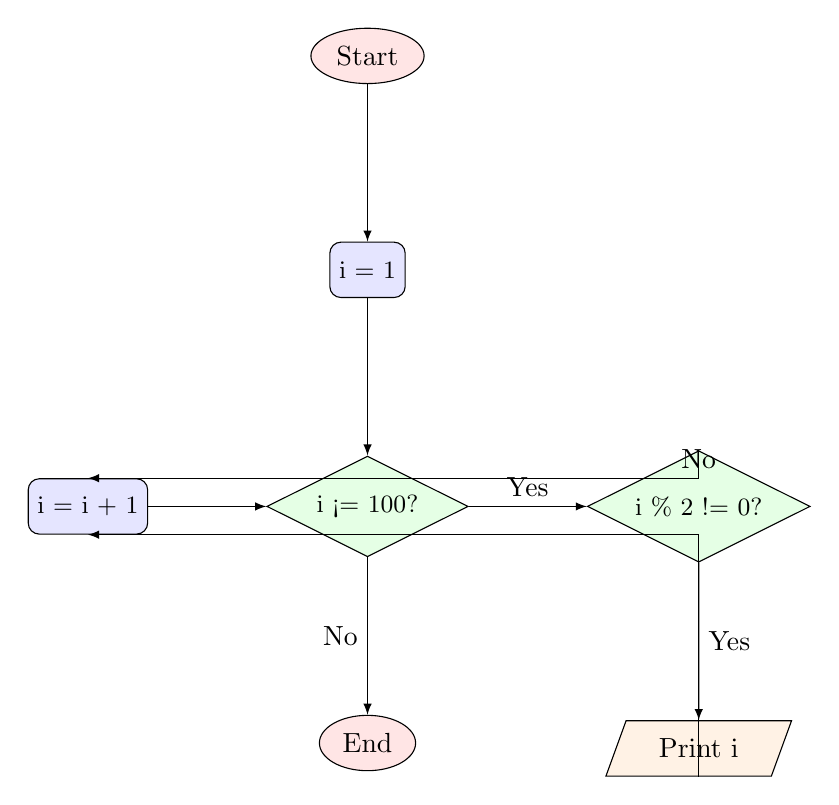
\begin{tikzpicture}[node distance=2cm, auto]
    \node[draw, ellipse, fill=red!10, align=center, minimum height=2em] (start) {Start};
    \node[rectangle, draw, fill=blue!10, align=center, rounded corners, minimum height=2em, font=\small, below=of start] (init) {i = 1};
    \node[diamond, draw, fill=green!10, align=center, aspect=2, font=\small, below=of init] (cond_loop) {i <= 100?};
    \node[diamond, draw, fill=green!10, align=center, aspect=2, font=\small, right=1.5cm of cond_loop] (cond_odd) {i \% 2 != 0?};
    \node[trapezium, trapezium left angle=70, trapezium right angle=110, draw, fill=orange!10, align=center, minimum height=2em, below=of cond_odd] (print) {Print i};
    \node[rectangle, draw, fill=blue!10, align=center, rounded corners, minimum height=2em, font=\small, left=1.5cm of cond_loop] (inc) {i = i + 1};
    \node[draw, ellipse, fill=red!10, align=center, minimum height=2em, below=of cond_loop] (stop) {End};

    \draw[draw, -latex] (start) -- (init);
    \draw[draw, -latex] (init) -- (cond_loop);
    \draw[draw, -latex] (cond_loop) -- node[above] {Yes} (cond_odd);
    \draw[draw, -latex] (cond_loop) -- node[left] {No} (stop);
    
    \draw[draw, -latex] (cond_odd) -- node[right] {Yes} (print);
    \draw[draw, -latex] (cond_odd.north) |- node[above] {No} (inc.north);
    
    \draw[draw, -latex] (print.south) |- (inc.south);
    \draw[draw, -latex] (inc) -- (cond_loop);
\end{tikzpicture}
\end{center}

\textbf{Corresponding Python Code:}
\begin{lstlisting}[language=Python]
for i in range(1, 101):
    if i % 2 != 0:
        print(i, end=" ")
\end{lstlisting}

\textbf{Alternative Method:}
\begin{lstlisting}[language=Python]
for i in range(1, 101, 2):
    print(i, end=" ")
\end{lstlisting}

\textbf{Key Elements:}
\begin{itemize}
    \item \textbf{Loop control}: i from 1 to 100
    \item \textbf{Odd check}: i \% 2 != 0 condition
    \item \textbf{Step increment}: Move to next number
\end{itemize}

\begin{mnemonicbox}\mnemonic{Odd Numbers: Remainder 1 When Divided by 2}\end{mnemonicbox}
\end{solutionbox}

\questionmarks{Question 2(a)}{03}{Write a Program to find whether a number is Palindrome or not.}

\begin{solutionbox}
\textbf{Palindrome Check Program:}
\begin{lstlisting}[language=Python]
# Input number
num = int(input("Enter a number: "))
temp = num
reverse = 0

# Reverse the number
while temp > 0:
    reverse = reverse * 10 + temp % 10
    temp = temp // 10

# Check palindrome
if num == reverse:
    print(f"{num} is palindrome")
else:
    print(f"{num} is not palindrome")
\end{lstlisting}

\textbf{Algorithm Table:}
\begin{answertable}{Algorithm Steps}
\begin{tabulary}{\linewidth}{|l|l|l|}
\hline
\textbf{Step} & \textbf{Operation} & \textbf{Example (121)} \\
\hline
1 & Get last digit & 121 \% 10 = 1 \\
\hline
2 & Build reverse & 0*10 + 1 = 1 \\
\hline
3 & Remove last digit & 121 // 10 = 12 \\
\hline
4 & Repeat until 0 & Continue process \\
\hline
\end{tabulary}
\end{answertable}

\textbf{Key Points:}
\begin{itemize}
    \item \textbf{Digit extraction}: Use modulo (\%) operator
    \item \textbf{Reverse building}: Multiply by 10 and add digit
    \item \textbf{Comparison}: Original equals reversed
\end{itemize}

\begin{mnemonicbox}\mnemonic{Palindrome Reads Same Forward Backward}\end{mnemonicbox}
\end{solutionbox}

\questionmarks{Question 2(b)}{04}{Explain features of Python Programming.}

\begin{solutionbox}
\textbf{Python Features Table:}
\begin{answertable}{Python Features}
\begin{tabulary}{\linewidth}{|l|l|l|}
\hline
\textbf{Feature} & \textbf{Description} & \textbf{Benefit} \\
\hline
Easy Syntax & Simple, readable code & Faster development \\
\hline
Interpreted & No compilation needed & Quick testing \\
\hline
Object-Oriented & Classes and objects support & Code reusability \\
\hline
Open Source & Free to use & No licensing cost \\
\hline
Cross-Platform & Runs on multiple OS & Wide compatibility \\
\hline
Large Libraries & Extensive built-in modules & Rich functionality \\
\hline
\end{tabulary}
\end{answertable}

\textbf{Key Advantages:}
\begin{itemize}
    \item \textbf{Beginner-friendly}: Easy to learn and understand
    \item \textbf{Versatile}: Web development, AI, data science
    \item \textbf{Community support}: Large developer community
    \item \textbf{Dynamic typing}: No variable type declaration needed
\end{itemize}

\begin{mnemonicbox}\mnemonic{Python: Easy, Powerful, Popular Programming}\end{mnemonicbox}
\end{solutionbox}

\questionmarks{Question 2(c)}{07}{Explain basic structure of Python Program.}

\begin{solutionbox}
\textbf{Python Program Structure:}
\begin{lstlisting}[language=Python]
#!/usr/bin/env python3
# Shebang line (optional)

"""
Documentation string (docstring)
Describes program purpose
"""

# Import statements
import math
from datetime import date

# Global variables
PI = 3.14159
count = 0

# Function definitions
def calculate_area(radius):
    """Calculate circle area"""
    return PI * radius * radius

# Class definitions
class Calculator:
    def __init__(self):
        self.result = 0

# Main program execution
if __name__ == "__main__":
    # Program logic here
    radius = 5
    area = calculate_area(radius)
    print(f"Area: {area}")
\end{lstlisting}

\textbf{Structure Components Table:}
\begin{answertable}{Program Components}
\begin{tabular}{|l|l|l|}
\hline
\textbf{Component} & \textbf{Purpose} & \textbf{Example} \\
\hline
Shebang & System interpreter & \code{\#!/usr/bin/env python3} \\
\hline
Docstring & Program documentation & \code{"""Program description"""} \\
\hline
Imports & External modules & \code{import math} \\
\hline
Variables & Global data storage & \code{PI = 3.14159} \\
\hline
Functions & Reusable code blocks & \code{def function\_name():} \\
\hline
\end{tabular}
\end{answertable}

\textbf{Key Principles:}
\begin{itemize}
    \item \textbf{Indentation}: Defines code blocks (4 spaces recommended)
    \item \textbf{Comments}: Use \# for single line, """ """ for multi-line
    \item \textbf{Modularity}: Organize code in functions and classes
\end{itemize}

\begin{mnemonicbox}\mnemonic{Structure: Import, Define, Execute}\end{mnemonicbox}
\end{solutionbox}

\questionmarks{Question 2(a OR)}{03}{Write a Program to reverse a string.}

\begin{solutionbox}
\textbf{String Reversal Program:}
\begin{lstlisting}[language=Python]
# Method 1: Using slicing
string = input("Enter a string: ")
reversed_string = string[::-1]
print(f"Reversed: {reversed_string}")

# Method 2: Using loop
string = input("Enter a string: ")
reversed_string = ""
for char in string:
    reversed_string = char + reversed_string
print(f"Reversed: {reversed_string}")
\end{lstlisting}

\textbf{Reversal Methods Table:}
\begin{answertable}{Reversal Methods}
\begin{tabulary}{\linewidth}{|l|l|l|}
\hline
\textbf{Method} & \textbf{Syntax} & \textbf{Example} \\
\hline
Slicing & \code{string[::-1]} & "hello" \rightarrow "olleh" \\
\hline
Loop & Build character by character & Add each char to front \\
\hline
Built-in & \code{"".join(reversed(string))} & Join reversed sequence \\
\hline
\end{tabulary}
\end{answertable}

\begin{mnemonicbox}\mnemonic{Reverse: Last Character First}\end{mnemonicbox}
\end{solutionbox}

\questionmarks{Question 2(b OR)}{04}{Explain Logical Operators with example.}

\begin{solutionbox}
\textbf{Python Logical Operators:}
\begin{answertable}{Logical Operators}
\begin{tabulary}{\linewidth}{|l|l|L|l|l|}
\hline
\textbf{Operator} & \textbf{Symbol} & \textbf{Description} & \textbf{Example} & \textbf{Result} \\
\hline
AND & \code{and} & Both conditions true & \code{True and False} & \code{False} \\
\hline
OR & \code{or} & At least one condition true & \code{True or False} & \code{True} \\
\hline
NOT & \code{not} & Opposite of condition & \code{not True} & \code{False} \\
\hline
\end{tabulary}
\end{answertable}

\textbf{Example Code:}
\begin{lstlisting}[language=Python]
a = 10
b = 5

# AND operator
if a > 5 and b < 10:
    print("Both conditions true")

# OR operator  
if a > 15 or b < 10:
    print("At least one condition true")

# NOT operator
if not (a < 5):
    print("a is not less than 5")
\end{lstlisting}

\textbf{Truth Table:}
\begin{answertable}{Truth Table}
\begin{tabulary}{\linewidth}{|c|c|c|c|c|}
\hline
\textbf{A} & \textbf{B} & \textbf{A and B} & \textbf{A or B} & \textbf{not A} \\
\hline
T & T & T & T & F \\
\hline
T & F & F & T & F \\
\hline
F & T & F & T & T \\
\hline
F & F & F & F & T \\
\hline
\end{tabulary}
\end{answertable}

\begin{mnemonicbox}\mnemonic{AND needs All, OR needs One, NOT reverses}\end{mnemonicbox}
\end{solutionbox}

\questionmarks{Question 2(c OR)}{07}{Explain different Data Types in Python Programming language}

\begin{solutionbox}
\textbf{Python Data Types Classification:}

\begin{center}
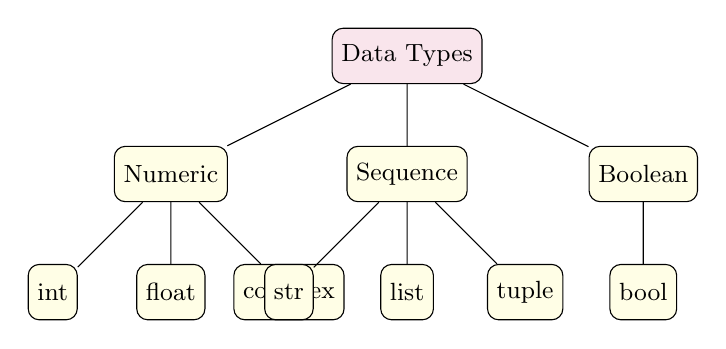
\begin{tikzpicture}[grow=down, level 1/.style={sibling distance=3cm}, level 2/.style={sibling distance=1.5cm}]
    \node[rectangle, draw, fill=blue!10, align=center, rounded corners, minimum height=2em, font=\small, fill=purple!10] {Data Types}
    child { node[rectangle, draw, fill=blue!10, align=center, rounded corners, minimum height=2em, font=\small, fill=yellow!10] {Numeric}
        child { node[rectangle, draw, fill=blue!10, align=center, rounded corners, minimum height=2em, font=\small, fill=yellow!10] {int} }
        child { node[rectangle, draw, fill=blue!10, align=center, rounded corners, minimum height=2em, font=\small, fill=yellow!10] {float} }
        child { node[rectangle, draw, fill=blue!10, align=center, rounded corners, minimum height=2em, font=\small, fill=yellow!10] {complex} }
    }
    child { node[rectangle, draw, fill=blue!10, align=center, rounded corners, minimum height=2em, font=\small, fill=yellow!10] {Sequence}
        child { node[rectangle, draw, fill=blue!10, align=center, rounded corners, minimum height=2em, font=\small, fill=yellow!10] {str} }
        child { node[rectangle, draw, fill=blue!10, align=center, rounded corners, minimum height=2em, font=\small, fill=yellow!10] {list} }
        child { node[rectangle, draw, fill=blue!10, align=center, rounded corners, minimum height=2em, font=\small, fill=yellow!10] {tuple} }
    }
    child { node[rectangle, draw, fill=blue!10, align=center, rounded corners, minimum height=2em, font=\small, fill=yellow!10] {Boolean}
        child { node[rectangle, draw, fill=blue!10, align=center, rounded corners, minimum height=2em, font=\small, fill=yellow!10] {bool} }
    };
\end{tikzpicture}
\end{center}

\textbf{Data Types Table:}
\begin{answertable}{Data Types}
\begin{tabulary}{\linewidth}{|l|l|l|l|}
\hline
\textbf{Type} & \textbf{Example} & \textbf{Description} & \textbf{Mutable} \\
\hline
int & \code{42} & Whole numbers & No \\
\hline
float & \code{3.14} & Decimal numbers & No \\
\hline
str & \code{"hello"} & Text data & No \\
\hline
list & \code{[1,2,3]} & Ordered collection & Yes \\
\hline
tuple & \code{(1,2,3)} & Ordered immutable & No \\
\hline
dict & \code{\{"a":1\}} & Key-value pairs & Yes \\
\hline
bool & \code{True/False} & Boolean values & No \\
\hline
set & \code{\{1,2,3\}} & Unique elements & Yes \\
\hline
\end{tabulary}
\end{answertable}

\textbf{Example Code:}
\begin{lstlisting}[language=Python]
# Numeric types
age = 25          # int
price = 99.99     # float
complex_num = 3+4j # complex

# Sequence types
name = "Python"         # string
numbers = [1,2,3,4]     # list
coordinates = (10,20)   # tuple

# Other types
is_active = True        # boolean
unique_items = {1,2,3}  # set
student = {"name":"John", "age":20}  # dict
\end{lstlisting}

\begin{mnemonicbox}\mnemonic{Python Types: Numbers, Sequences, Collections}\end{mnemonicbox}
\end{solutionbox}

\questionmarks{Question 3(a)}{03}{What is flow control in Python? Explain with example}

\begin{solutionbox}
\textbf{Flow control} manages the execution order of program statements using conditional and loop structures.

\textbf{Flow Control Types Table:}
\begin{answertable}{Flow Control Types}
\begin{tabulary}{\linewidth}{|l|l|l|l|}
\hline
\textbf{Type} & \textbf{Statement} & \textbf{Purpose} & \textbf{Example} \\
\hline
Sequential & Normal execution & Line by line & \code{print("Hello")} \\
\hline
Selection & if, elif, else & Decision making & \code{if x > 0:} \\
\hline
Iteration & for, while & Repetition & \code{for i in range(5):} \\
\hline
Jump & break, continue & Loop control & \code{break} \\
\hline
\end{tabulary}
\end{answertable}

\textbf{Example Code:}
\begin{lstlisting}[language=Python]
# Selection example
age = 18
if age >= 18:
    print("Adult")
else:
    print("Minor")

# Iteration example
for i in range(3):
    print(f"Count: {i}")
\end{lstlisting}

\begin{mnemonicbox}\mnemonic{Flow Control: Decide, Repeat, Jump}\end{mnemonicbox}
\end{solutionbox}

\questionmarks{Question 3(b)}{04}{Write a program to explain nested if statement.}

\begin{solutionbox}
\textbf{Nested If Statement Program:}
\begin{lstlisting}[language=Python]
# Grade calculation using nested if
marks = int(input("Enter marks: "))

if marks >= 0 and marks <= 100:
    if marks >= 90:
        grade = "A+"
    elif marks >= 80:
        if marks >= 85:
            grade = "A"
        else:
            grade = "B+"
    elif marks >= 70:
        grade = "B"
    elif marks >= 60:
        grade = "C"
    else:
        grade = "F"
    print(f"Grade: {grade}")
else:
    print("Invalid marks")
\end{lstlisting}

\textbf{Nested Structure Diagram:}
\begin{center}
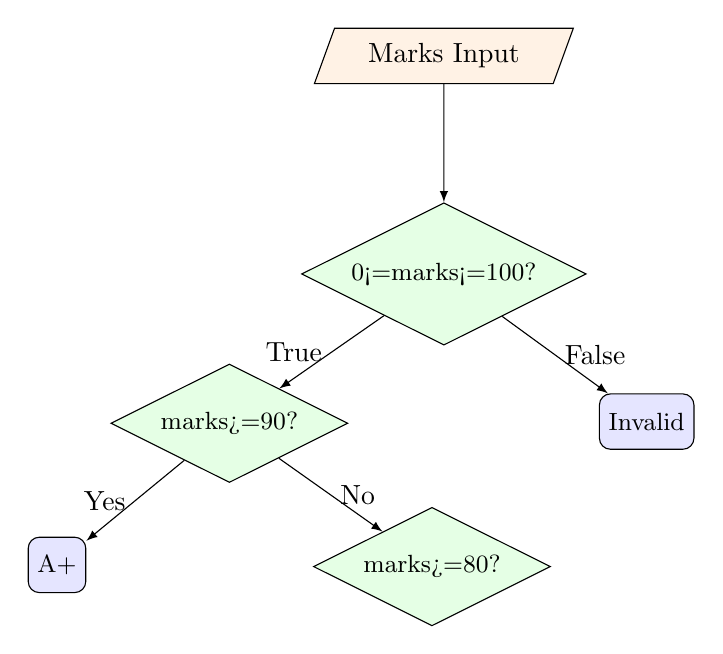
\begin{tikzpicture}[node distance=1.5cm, auto]
    \node[trapezium, trapezium left angle=70, trapezium right angle=110, draw, fill=orange!10, align=center, minimum height=2em] (input) {Marks Input};
    \node[diamond, draw, fill=green!10, align=center, aspect=2, font=\small, below=of input] (range) {0<=marks<=100?};
    \node[diamond, draw, fill=green!10, align=center, aspect=2, font=\small, below left=of range] (grade90) {marks>=90?};
    \node[rectangle, draw, fill=blue!10, align=center, rounded corners, minimum height=2em, font=\small, below right=of range] (invalid) {Invalid};
    
    \node[rectangle, draw, fill=blue!10, align=center, rounded corners, minimum height=2em, font=\small, below left=of grade90] (Ap) {A+};
    \node[diamond, draw, fill=green!10, align=center, aspect=2, font=\small, below right=of grade90] (grade80) {marks>=80?};

    \draw[draw, -latex] (input) -- (range);
    \draw[draw, -latex] (range) -- node[left] {True} (grade90);
    \draw[draw, -latex] (range) -- node[right] {False} (invalid);
    \draw[draw, -latex] (grade90) -- node[left] {Yes} (Ap);
    \draw[draw, -latex] (grade90) -- node[right] {No} (grade80);
\end{tikzpicture}
\end{center}

\begin{mnemonicbox}\mnemonic{Nested If: Decisions Within Decisions}\end{mnemonicbox}
\end{solutionbox}

\questionmarks{Question 3(c)}{07}{Write a program to Explain types of Arguments and Parameters.}

\begin{solutionbox}
\textbf{Types of Arguments and Parameters:}
\begin{lstlisting}[language=Python]
# 1. Positional Arguments
def greet(name, age):
    print(f"Hello {name}, you are {age} years old")

greet("John", 25)  # Positional arguments

# 2. Keyword Arguments  
greet(age=30, name="Alice")  # Keyword arguments

# 3. Default Parameters
def introduce(name, city="Unknown"):
    print(f"{name} lives in {city}")

introduce("Bob")  # Uses default value
introduce("Carol", "NYC")  # Override default

# 4. Variable-length Arguments (*args)
def sum_all(*numbers):
    return sum(numbers)

result = sum_all(1, 2, 3, 4, 5)
print(f"Sum: {result}")

# 5. Keyword Variable Arguments (**kwargs)
def display_info(**info):
    for key, value in info.items():
        print(f"{key}: {value}")

display_info(name="David", age=28, city="Boston")
\end{lstlisting}

\textbf{Parameters Types Table:}
\begin{answertable}{Parameter Types}
\begin{tabulary}{\linewidth}{|l|l|l|l|}
\hline
\textbf{Type} & \textbf{Syntax} & \textbf{Example} & \textbf{Description} \\
\hline
Positional & \code{def func(a, b):} & \code{func(1, 2)} & Order matters \\
\hline
Keyword & \code{def func(a, b):} & \code{func(b=2, a=1)} & Name specified \\
\hline
Default & \code{def func(a, b=10):} & \code{func(5)} & Default value \\
\hline
*args & \code{def func(*args):} & \code{func(1,2,3)} & Variable positional \\
\hline
**kwargs & \code{def func(**kwargs):} & \code{func(a=1, b=2)} & Variable keyword \\
\hline
\end{tabulary}
\end{answertable}

\begin{mnemonicbox}\mnemonic{Parameters: Position, Keywords, Defaults, Variables}\end{mnemonicbox}
\end{solutionbox}

\questionmarks{Question 3(a OR)}{03}{Explain break and continue statement with example.}

\begin{solutionbox}
\textbf{Break and Continue Statements:}

\textbf{Break Statement:}
\begin{lstlisting}[language=Python]
# Break example - exit loop
for i in range(10):
    if i == 5:
        break
    print(i)
# Output: 0, 1, 2, 3, 4
\end{lstlisting}

\textbf{Continue Statement:}
\begin{lstlisting}[language=Python]
# Continue example - skip iteration
for i in range(5):
    if i == 2:
        continue
    print(i)
# Output: 0, 1, 3, 4
\end{lstlisting}

\textbf{Comparison Table:}
\begin{answertable}{Break vs Continue}
\begin{tabulary}{\linewidth}{|l|l|l|l|}
\hline
\textbf{Statement} & \textbf{Purpose} & \textbf{Action} & \textbf{Example Use} \\
\hline
break & Exit loop & Terminates entire loop & Exit on condition \\
\hline
continue & Skip iteration & Jump to next iteration & Skip specific values \\
\hline
\end{tabulary}
\end{answertable}

\begin{mnemonicbox}\mnemonic{Break Exits, Continue Skips}\end{mnemonicbox}
\end{solutionbox}

\questionmarks{Question 3(b OR)}{04}{Create a program to display the following pattern}

\begin{solutionbox}
\textbf{Pattern:}
\begin{verbatim}
1
12
123
1234
12345
\end{verbatim}

\textbf{Number Pattern Program:}
\begin{lstlisting}[language=Python]
# Method 1: Using nested loops
rows = 5
for i in range(1, rows + 1):
    for j in range(1, i + 1):
        print(j, end="")
    print()  # New line
    
# Method 2: Using string manipulation
for i in range(1, 6):
    line = ""
    for j in range(1, i + 1):
        line += str(j)
    print(line)
\end{lstlisting}

\begin{mnemonicbox}\mnemonic{Pattern: Row Number Determines Column Count}\end{mnemonicbox}
\end{solutionbox}

\questionmarks{Question 3(c OR)}{07}{Explain the following mathematical functions by writing a code for each: 1. abs() 2. max() 3. pow() 4. sum()}

\begin{solutionbox}
\textbf{Mathematical Functions in Python:}
\begin{lstlisting}[language=Python]
# 1. abs() - Absolute value
numbers = [-5, 3.7, -10.2, 0]
print("abs() function examples:")
for num in numbers:
    print(f"abs({num}) = {abs(num)}")

# 2. max() - Maximum value
list1 = [4, 7, 2, 9, 1]
print(f"\nmax() function examples:")
print(f"max({list1}) = {max(list1)}")
print(f"max(10, 25, 5) = {max(10, 25, 5)}")
print(f"max('hello') = {max('hello')}")  # Alphabetically

# 3. pow() - Power function
print(f"\npow() function examples:")
print(f"pow(2, 3) = {pow(2, 3)}")      # 2^3 = 8
print(f"pow(5, 2) = {pow(5, 2)}")      # 5^2 = 25
print(f"pow(8, 1/3) = {pow(8, 1/3)}")  # Cube root of 8

# 4. sum() - Sum of sequence
numbers = [1, 2, 3, 4, 5]
print(f"\nsum() function examples:")
print(f"sum({numbers}) = {sum(numbers)}")
print(f"sum({numbers}, 10) = {sum(numbers, 10)}")  # With start value
\end{lstlisting}

\textbf{Functions Summary Table:}
\begin{answertable}{Math Functions}
\begin{tabulary}{\linewidth}{|l|l|l|l|l|}
\hline
\textbf{Function} & \textbf{Syntax} & \textbf{Purpose} & \textbf{Example} & \textbf{Result} \\
\hline
abs() & \code{abs(x)} & Absolute value & \code{abs(-5)} & 5 \\
\hline
max() & \code{max(iterable)} & Maximum value & \code{max([1,5,3])} & 5 \\
\hline
pow() & \code{pow(x, y)} & x raised to power y & \code{pow(2, 3)} & 8 \\
\hline
sum() & \code{sum(iterable)} & Sum of values & \code{sum([1,2,3])} & 6 \\
\hline
\end{tabulary}
\end{answertable}

\begin{mnemonicbox}\mnemonic{Math Functions: Absolute, Maximum, Power, Sum}\end{mnemonicbox}
\end{solutionbox}

\questionmarks{Question 4(a)}{03}{Explain scope of variables.}

\begin{solutionbox}
\textbf{Variable Scope} refers to the region where a variable can be accessed in a program.

\textbf{Scope Types Table:}
\begin{answertable}{Variable Scope}
\begin{tabulary}{\linewidth}{|l|l|l|l|}
\hline
\textbf{Scope} & \textbf{Description} & \textbf{Lifetime} & \textbf{Access} \\
\hline
Local & Inside function & Function execution & Function only \\
\hline
Global & Outside functions & Program execution & Entire program \\
\hline
Built-in & Python keywords & Python session & Everywhere \\
\hline
\end{tabulary}
\end{answertable}

\begin{mnemonicbox}\mnemonic{Scope: Local Lives in Functions, Global Lives Everywhere}\end{mnemonicbox}
\end{solutionbox}

\questionmarks{Question 4(b)}{04}{Develop a program to create nested LOOP and display numbers.}

\begin{solutionbox}
\textbf{Nested Loop Program:}
\begin{lstlisting}[language=Python]
# Example 1: Number grid
print("Number Grid Pattern:")
for i in range(1, 4):
    for j in range(1, 5):
        print(f"{i}{j}", end=" ")
    print()  # New line after each row
\end{lstlisting}

\textbf{Nested Loop Structure:}
\begin{center}
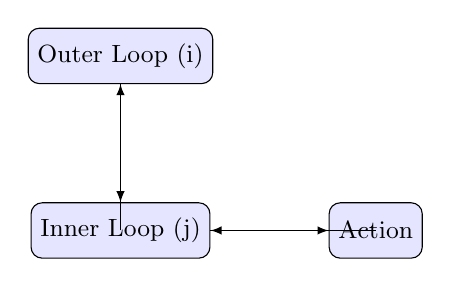
\begin{tikzpicture}[node distance=1.5cm, auto]
    \node[rectangle, draw, fill=blue!10, align=center, rounded corners, minimum height=2em, font=\small] (outer) {Outer Loop (i)};
    \node[rectangle, draw, fill=blue!10, align=center, rounded corners, minimum height=2em, font=\small, below=of outer] (inner) {Inner Loop (j)};
    \node[rectangle, draw, fill=blue!10, align=center, rounded corners, minimum height=2em, font=\small, right=of inner] (action) {Action};

    \draw[draw, -latex] (outer) -- (inner);
    \draw[draw, -latex] (inner) -- (action);
    \draw[draw, -latex] (action) |- (inner);
    \draw[draw, -latex] (inner) -| (outer);
\end{tikzpicture}
\end{center}

\begin{mnemonicbox}\mnemonic{Nested Loops: Outer Controls Inner}\end{mnemonicbox}
\end{solutionbox}

\questionmarks{Question 4(c)}{07}{Write a program to create a list of ODD and EVEN numbers in range of 1 to 50.}

\begin{solutionbox}
\textbf{ODD and EVEN Numbers Program:}
\begin{lstlisting}[language=Python]
# Method 1: Using loops and conditions
odd_numbers = []
even_numbers = []

for i in range(1, 51):
    if i % 2 == 0:
        even_numbers.append(i)
    else:
        odd_numbers.append(i)

print("ODD Numbers (1-50):")
print(odd_numbers)
print(f"Count: {len(odd_numbers)}")

print("\nEVEN Numbers (1-50):")
print(even_numbers)
print(f"Count: {len(even_numbers)}")
\end{lstlisting}

\textbf{Number Classification Table:}
\begin{answertable}{Number Classification}
\begin{tabulary}{\linewidth}{|l|l|l|l|}
\hline
\textbf{Type} & \textbf{Condition} & \textbf{Range 1-10} & \textbf{Count (1-50)} \\
\hline
ODD & \code{n \% 2 != 0} & 1,3,5,7,9 & 25 \\
\hline
EVEN & \code{n \% 2 == 0} & 2,4,6,8,10 & 25 \\
\hline
\end{tabulary}
\end{answertable}

\begin{mnemonicbox}\mnemonic{Odd/Even: Remainder 1/0 When Divided by 2}\end{mnemonicbox}
\end{solutionbox}

\questionmarks{Question 4(a OR)}{03}{Explain String Slicing with example.}

\begin{solutionbox}
\textbf{String Slicing} extracts parts of a string using \code{[start:stop:step]} syntax.

\textbf{Slicing Syntax Table:}
\begin{answertable}{Slicing Syntax}
\begin{tabulary}{\linewidth}{|l|l|l|l|}
\hline
\textbf{Syntax} & \textbf{Description} & \textbf{Example} & \textbf{Result} \\
\hline
\code{s[start:stop]} & From start to stop-1 & \code{"hello"[1:4]} & "ell" \\
\hline
\code{s[start:]} & From start to end & \code{"hello"[2:]} & "llo" \\
\hline
\code{s[:stop]} & From beginning to stop-1 & \code{"hello"[:3]} & "hel" \\
\hline
\code{s[::step]} & Every step character & \code{"hello"[::2]} & "hlo" \\
\hline
\code{s[::-1]} & Reverse string & \code{"hello"[::-1]} & "olleh" \\
\hline
\end{tabulary}
\end{answertable}

\begin{mnemonicbox}\mnemonic{Slice: Start, Stop, Step}\end{mnemonicbox}
\end{solutionbox}

\questionmarks{Question 4(b OR)}{04}{Write a program using user defined function to find the factorial of a given number.}

\begin{solutionbox}
\textbf{Factorial Function Program:}
\begin{lstlisting}[language=Python]
def factorial(n):
    """Calculate factorial using recursion"""
    if n == 0 or n == 1:
        return 1
    else:
        return n * factorial(n - 1)

def factorial_iterative(n):
    """Calculate factorial using loop"""
    result = 1
    for i in range(1, n + 1):
        result *= i
    return result

# Main program
number = int(input("Enter a number: "))
if number < 0:
    print("Factorial not defined for negative numbers")
else:
    result1 = factorial(number)
    print(f"Factorial of {number} = {result1}")
\end{lstlisting}

\begin{mnemonicbox}\mnemonic{Factorial: Multiply All Numbers Below}\end{mnemonicbox}
\end{solutionbox}

\questionmarks{Question 4(c OR)}{07}{Write a user defined function to check whether a sub string is present in a given string.}

\begin{solutionbox}
\textbf{Substring Check Function:}
\begin{lstlisting}[language=Python]
def find_substring(main_string, sub_string):
    """Check if substring exists in main string"""
    if sub_string in main_string:
        index = main_string.find(sub_string)
        return True, index
    else:
        return False, -1

# Main program
text = input("Enter main string: ")
search = input("Enter substring to search: ")

found, position = find_substring(text, search)
if found:
    print(f"Substring '{search}' found at position {position}")
else:
    print(f"Substring '{search}' not found")
\end{lstlisting}

\textbf{String Methods Table:}
\begin{answertable}{String Methods}
\begin{tabulary}{\linewidth}{|l|l|l|l|}
\hline
\textbf{Method} & \textbf{Purpose} & \textbf{Example} & \textbf{Result} \\
\hline
\code{find()} & Find first position & \code{"hello".find("ll")} & 2 \\
\hline
\code{count()} & Count occurrences & \code{"hello".count("l")} & 2 \\
\hline
\code{in} & Check existence & \code{"ll" in "hello"} & True \\
\hline
\code{index()} & Find position (error if not found) & \code{"hello".index("e")} & 1 \\
\hline
\end{tabulary}
\end{answertable}

\begin{mnemonicbox}\mnemonic{Substring: Search, Find, Count, Position}\end{mnemonicbox}
\end{solutionbox}

\questionmarks{Question 5(a)}{03}{Explain how to create and access a List with example.}

\begin{solutionbox}
\textbf{List Creation and Access:}
\begin{lstlisting}[language=Python]
# Creating lists
numbers = [1, 2, 3, 4, 5]

# Accessing elements
print(f"First element: {numbers[0]}")      # 1
print(f"Last element: {numbers[-1]}")      # 5
print(f"Slice: {numbers[1:4]}")           # [2, 3, 4]
\end{lstlisting}

\textbf{List Access Methods:}
\begin{answertable}{List Access}
\begin{tabulary}{\linewidth}{|l|l|l|l|}
\hline
\textbf{Method} & \textbf{Syntax} & \textbf{Example} & \textbf{Result} \\
\hline
Index & \code{list[i]} & \code{[1,2,3][1]} & 2 \\
\hline
Negative & \code{list[-i]} & \code{[1,2,3][-1]} & 3 \\
\hline
Slice & \code{list[start:stop]} & \code{[1,2,3,4][1:3]} & [2,3] \\
\hline
\end{tabulary}
\end{answertable}

\begin{mnemonicbox}\mnemonic{Lists: Create, Index, Access}\end{mnemonicbox}
\end{solutionbox}

\questionmarks{Question 5(b)}{04}{List out the operations that can be performed on a LIST. Write a program to create and copy one List into another List.}

\begin{solutionbox}
\textbf{List Operations and Copy Program:}
\begin{lstlisting}[language=Python]
# Original list
original = [1, 2, 3, 4, 5]
print(f"Original list: {original}")

# Copying methods
shallow_copy = original.copy()
slice_copy = original[:]
list_copy = list(original)

# Modify original
original.append(6)
print(f"After append: {original}")
print(f"Shallow copy: {shallow_copy}")
\end{lstlisting}

\textbf{List Operations Table:}
\begin{answertable}{List Operations}
\begin{tabulary}{\linewidth}{|l|l|l|l|}
\hline
\textbf{Operation} & \textbf{Method} & \textbf{Example} & \textbf{Result} \\
\hline
Add & \code{append()} & \code{[1,2].append(3)} & [1,2,3] \\
\hline
Insert & \code{insert()} & \code{[1,3].insert(1,2)} & [1,2,3] \\
\hline
Remove & \code{remove()} & \code{[1,2,3].remove(2)} & [1,3] \\
\hline
Pop & \code{pop()} & \code{[1,2,3].pop()} & [1,2] \\
\hline
\end{tabulary}
\end{answertable}

\begin{mnemonicbox}\mnemonic{List Operations: Add, Insert, Remove, Pop, Copy}\end{mnemonicbox}
\end{solutionbox}

\questionmarks{Question 5(c)}{07}{List and give use of various Built in methods of LIST}

\begin{solutionbox}
\textbf{Built-in List Methods:}
\begin{lstlisting}[language=Python]
# Sample list for demonstrations
fruits = ['apple', 'banana', 'cherry', 'apple']

# Modification methods
fruits.append('date')              # Add to end
fruits.insert(1, 'avocado')       # Insert at index
fruits.remove('apple')            # Remove first occurrence
last_fruit = fruits.pop()         # Remove and return last

# Search and count methods
count = fruits.count('apple')     # Count occurrences
index = fruits.index('banana')    # Find first index

# Sorting and reversing
fruits.sort()                     # Sort in place
fruits.reverse()                  # Reverse in place
\end{lstlisting}

\textbf{List Methods Summary:}
\begin{answertable}{List Methods}
\begin{tabulary}{\linewidth}{|l|l|l|l|l|}
\hline
\textbf{Category} & \textbf{Method} & \textbf{Purpose} & \textbf{Returns} & \textbf{Modifies Original} \\
\hline
Add & \code{append(x)} & Add item to end & None & Yes \\
\hline
Add & \code{insert(i,x)} & Insert at position & None & Yes \\
\hline
Remove & \code{remove(x)} & Remove first x & None & Yes \\
\hline
Remove & \code{pop(i)} & Remove at index & Removed item & Yes \\
\hline
Search & \code{index(x)} & Find position & Index & No \\
\hline
Sort & \code{sort()} & Sort in place & None & Yes \\
\hline
Sort & \code{reverse()} & Reverse order & None & Yes \\
\hline
Copy & \code{copy()} & Shallow copy & New list & No \\
\hline
\end{tabulary}
\end{answertable}

\begin{mnemonicbox}\mnemonic{List Methods: Add, Remove, Search, Sort, Copy}\end{mnemonicbox}
\end{solutionbox}

\questionmarks{Question 5(a OR)}{03}{Explain how to create and traverse a string by giving an example.}

\begin{solutionbox}
\textbf{String Creation and Traversal:}
\begin{lstlisting}[language=Python]
# String creation methods
string1 = "Hello World"        # Double quotes
string2 = 'Python'             # Single quotes

# String traversal methods
text = "Python"

# Method 1: Using for loop
for char in text:
    print(char, end=" ")
\end{lstlisting}

\textbf{Traversal Methods Table:}
\begin{answertable}{Traversal Methods}
\begin{tabulary}{\linewidth}{|l|l|l|}
\hline
\textbf{Method} & \textbf{Syntax} & \textbf{Use Case} \\
\hline
Direct & \code{for char in string:} & Simple character access \\
\hline
Index & \code{for i in range(len(s)):} & Need position info \\
\hline
Enumerate & \code{for i, char in enumerate(s):} & Both index and character \\
\hline
\end{tabulary}
\end{answertable}

\begin{mnemonicbox}\mnemonic{Strings: Create, Loop, Access}\end{mnemonicbox}
\end{solutionbox}

\questionmarks{Question 5(b OR)}{04}{List out the operations that can be performed on a String. Write a code for any 2 operations}

\begin{solutionbox}
\textbf{String Operations:}
\begin{lstlisting}[language=Python]
# Operation 1: String concatenation
first_name = "John"
last_name = "Doe"
full_name = first_name + " " + last_name
print(f"Concatenation: {full_name}")

# Operation 2: String case conversion
sentence = "learn python"
title_case = sentence.title()
print(f"Title case: {title_case}")
\end{lstlisting}

\textbf{String Operations Table:}
\begin{answertable}{String Operations}
\begin{tabulary}{\linewidth}{|l|l|l|l|}
\hline
\textbf{Category} & \textbf{Operation} & \textbf{Example} & \textbf{Result} \\
\hline
Join & Concatenation & \code{"Hello" + " World"} & "Hello World" \\
\hline
Case & \code{upper()} & \code{"hello".upper()} & "HELLO" \\
\hline
Case & \code{lower()} & \code{"HELLO".lower()} & "hello" \\
\hline
Split & \code{split()} & \code{"a,b".split(",")} & ['a','b'] \\
\hline
Replace & \code{replace()} & \code{"hi".replace("i","o")} & "ho" \\
\hline
\end{tabulary}
\end{answertable}

\begin{mnemonicbox}\mnemonic{String Operations: Join, Case, Split, Find}\end{mnemonicbox}
\end{solutionbox}

\questionmarks{Question 5(c OR)}{07}{List and give use of various built – in methods of String.}

\begin{solutionbox}
\textbf{Built-in String Methods:}
\begin{lstlisting}[language=Python]
# Sample string for demonstration
text = "  Python Programming  "

# Case conversion methods
print(f"upper(): {text.upper()}")
print(f"lower(): {text.lower()}")

# Whitespace methods
print(f"strip(): '{text.strip()}'")

# Search and check methods
print(f"find('Python'): {text.find('Python')}")
print(f"count('P'): {text.count('P')}")

# Split and join methods
words = text.split()
print(f"split(): {words}")
\end{lstlisting}

\textbf{String Methods Classification:}
\begin{answertable}{String Methods Class}
\begin{tabulary}{\linewidth}{|l|l|l|l|}
\hline
\textbf{Category} & \textbf{Methods} & \textbf{Purpose} & \textbf{Example} \\
\hline
Case & \code{upper(), lower()} & Change case & \code{"hi".upper()} \rightarrow "HI" \\
\hline
Whitespace & \code{strip()} & Remove spaces & \code{" h ".strip()} \rightarrow "h" \\
\hline
Search & \code{find(), count()} & Find substrings & \code{"hi".find("i")} \rightarrow 1 \\
\hline
Check & \code{startswith()} & Test string ends & \code{"hi".startswith("h")} \rightarrow True \\
\hline
Type Check & \code{isdigit()} & Character types & \code{"1".isdigit()} \rightarrow True \\
\hline
Replace & \code{replace()} & Substitute text & \code{"sub".replace("u","o")} \rightarrow "sob" \\
\hline
\end{tabulary}
\end{answertable}

\begin{mnemonicbox}\mnemonic{String Methods: Case, Clean, Check, Change}\end{mnemonicbox}
\end{solutionbox}

\end{document}
